\section{Vistas}\label{sec:vistas}

\begin{quote}
\textbf{In plain words.} The same rules, applied to the sky. Close to a pair of
black holes the camera would see them as two, turning; farther out it sees
only the spiral of their waves. An exploding star is invisible unless it is
lopsided, and then it leaves space permanently stretched. The Milky Way's
centre, hidden from light behind dust, is the brightest thing in the
gravitational sky. And if the Big Bang was ever hot enough, the whole sky
glows at a temperature just under one kelvin, a background against which the
only shadows are black holes.
\end{quote}

The scenes so far are rooms and planets. This section follows the same
equations to the scales where they are most striking. We chose problems that
have exact or closed-form solutions, so that every picture below is computed
from physics, not drawn; each is checked by tests in the reference
implementation. The website lets the reader look around three of these skies
live.

\paragraph{A pair of black holes, from the inside out.} Outside any compact
source, linearized gravity has an exact solution organised by multipoles
\cite{Thorne1980}. Kept to the order of the mass quadrupole $I_{ij}$, with
$u = t - r/c$ and $\hat n$ the direction from the source, the trace-reversed
perturbation in harmonic gauge is
\begin{equation}\label{eq:multipole}
\begin{aligned}
\bar h^{00} &= \frac{4G}{c^2}\Bigl[\frac{M}{r} + \frac{1}{2}\,\partial_i\partial_j\frac{I_{ij}(u)}{r}\Bigr],\\
\bar h^{0i} &= \frac{2G}{c^3}\Bigl[\frac{\dot I_{ij}(u)\,\hat n_j}{r^2} + \frac{\ddot I_{ij}(u)\,\hat n_j}{c\,r}
+ \frac{(\mathbf J\times\mathbf x)_i}{r^3}\Bigr],\\
\bar h^{ij} &= \frac{2G}{c^4}\,\frac{\ddot I_{ij}(u)}{r},
\end{aligned}
\end{equation}
with $M$ the mass, $\mathbf J$ the angular momentum and $I_{ij} = \int\rho\,
x_ix_j\,\dd^3x$ the second moment of the mass, its trace included (outside
the source the trace changes only the gauge, not the curvature, as the
reference implementation confirms). It satisfies the gauge condition exactly,
and its curvature gives the tidal field in every zone at once
\cite{Teukolsky1982}: exactly, within linearized gravity and this truncation
of the multipoles. Figure~\ref{fig:binary-field} shows it in the plane
of an orbit, for two black holes of thirty solar masses each about ten seconds
before they merge, when they are $2200\,\mathrm{km}$ apart and move at a tenth
of the speed of light; their waves are $35{,}000\,\mathrm{km}$ long. Within a
reduced wavelength, $\lambda/2\pi$, the changing part of the field is Newton's
pull of two masses, turning rigidly with them and falling as $r^{-5}$. Beyond
it the pattern winds into a two-armed spiral whose strength falls only as
$r^{-1}$: the waves. The two meet where
$G\,\Delta I/r^5 \approx G\,\Delta I\,\omega^4/c^4 r$, that is at
$r \approx c/\omega = \lambda/2\pi$.

This marks a crossover between the two ways the camera sees, not a sharp
edge. Well inside it the near-field imaging of Section~\ref{sec:near-field}
applies, and an array could resolve the pair as two bodies, if its
signal-to-noise ratio and width meet the blur law there; well outside it,
Eq.~\eqref{eq:unresolved} holds and the pair is a point whose polarization
tells the axis and sense of its orbit. Being within about a sixth of a
wavelength is needed to see two black holes as two, but it is not enough by
itself. The reference
implementation computes the field of Eq.~\eqref{eq:multipole} by finite
differences of the curvature and checks that it becomes Newton's field of the
two masses near them, with an error falling as $(d/r)^2$, and the quadrupole
wave far away, with an error falling as $\lambda/r$, and that it is the
curvature of vacuum, with $|\tB| = |\tE|$ in the waves.

\begin{figure*}
\centering
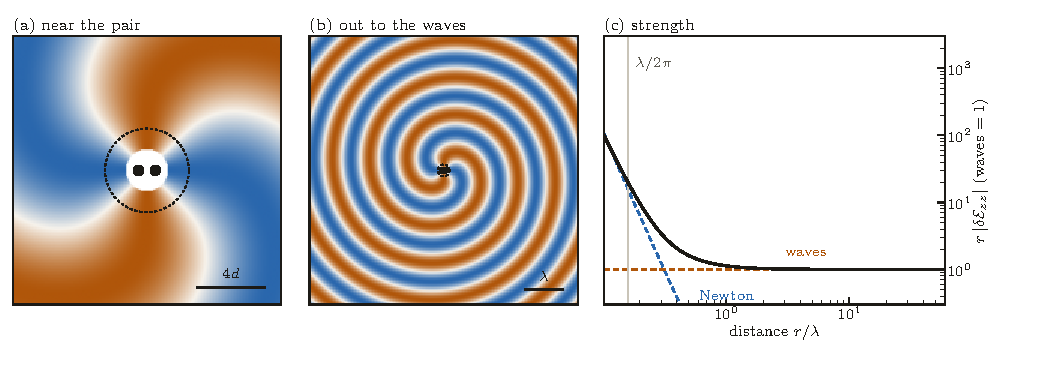
\includegraphics[width=\textwidth]{figures/binary-field.pdf}
\caption{Two black holes of thirty solar masses, ten seconds before they
merge, in the plane of their orbit: the changing part of the tidal field
$\tE_{zz}$ (across the plane), from the linearized solution of
Eq.~\eqref{eq:multipole}, exact within that model. Colour gives the phase, orange for stretch and blue
for squeeze, scaled at each place by the local strength. (a) Near the pair,
whose separation is $d$, the pattern turns rigidly with it; beyond the dashed
circle, $r = \lambda/2\pi$, it begins to wind. (b) Farther out it is the spiral
of the waves. (c) The strength along a line in the plane, times $r$: Newton's
$r^{-5}$ inside $\lambda/2\pi$, the waves' $r^{-1}$ outside. The field is an
exact solution of linearized gravity truncated at the mass quadrupole, which
this close to a merger is a guide to the full solution, not a substitute for
it.}\label{fig:binary-field}
\end{figure*}

\paragraph{What a burst leaves behind.} Radiation that escapes to infinity
carries away mass, and a camera it passes is left permanently deformed: the
memory \cite{Christodoulou1991,Thorne1992}. For energy radiated with angular
distribution $\dd E/\dd\Omega'$, at nearly the speed of light, the change in
strain seen from direction $\hat N$ at distance $r$ is
\cite{Epstein1978,Thorne1992}
\begin{equation}\label{eq:memory}
\Delta h_{ij}^{\TT} = \frac{4G}{c^4 r}\int \frac{\dd E}{\dd\Omega'}
\left[\frac{n'_i n'_j}{1 - \hat n'\cdot\hat N}\right]^{\TT}\dd\Omega' .
\end{equation}
Applied to the waves of a merger themselves, whose power goes as
$(1+\cos^2\iota)^2/4 + \cos^2\iota$, it gives
\begin{equation}\label{eq:merger-memory}
\Delta h_+ = \frac{G\,\Delta E}{24\,c^4 r}\,\sin^2\iota\,\bigl(17 + \cos^2\iota\bigr),
\end{equation}
the shape found by Wiseman and Will \cite{WisemanWill1991,Favata2009}, which
we reproduce by integrating Eq.~\eqref{eq:memory} numerically. It is largest
seen edge-on, where the oscillating wave is weakest (Figure~\ref{fig:memory}).
A camera that records the field, not the strain, sees the memory as a burst of
$\tE$ whose second time integral does not return to zero.

\paragraph{An exploding star.} A spherical collapse or explosion radiates
nothing: by Birkhoff's theorem the field outside a spherical body is that of a
point mass, whatever happens within. It does change once. A core collapse
sends out some $3\times10^{46}\,\mathrm{J}$ in neutrinos, a sixth of a solar
mass, as a thin shell moving at nearly the speed of light, and outside the
shell the field is that of the original mass, inside it that of the remnant
\cite{Vaidya1951}. A near-field camera sees the star lose the neutrinos'
mass at the moment the shell passes the camera, not before: it weighs the
burst as it arrives. While the shell passes, the camera also feels the
neutrinos themselves. Their flux of energy, $F = L/4\pi r^2$ at luminosity
$L$, enters the Ricci part of the curvature and squeezes the camera evenly
across their direction of travel, $\tE_{ij} = (GL/c^3r^2)(\delta_{ij} - \hat
n_i\hat n_j)$, while $\tB$ gains the antisymmetric part of
Section~\ref{sec:pixel}, set by their flow, so that one pixel points to the
star although the explosion is spherical. From ten kiloparsecs this squeeze,
while it lasts, is some $10^{11}$ times the change of pull it leaves behind. If the neutrinos leave unevenly the explosion also leaves
memory \cite{Epstein1978,Turner1978}. A narrow jet of energy $E$ leaves
$\Delta h = (2GE/c^4 r)(1 + \cos\theta)$ at angle $\theta$ from it, largest
just off the line it travels along (exactly on that line symmetry allows
none, and a jet of finite width turns the memory off within its own width
of the axis); two opposite jets leave the same $2GE/c^4 r$ in every
direction off their axis; a sphere leaves nothing (Figure~\ref{fig:memory}).
Only the quadrupole and higher parts of the pattern count: the radiation of a
burst that is merely brighter on one side, a pure dipole, leaves no memory at
all. It does push the star the other way, and the recoiling remnant leaves a
memory of its own, second order in the small recoil \cite{Favata2009}. A burst
stronger along an axis than across it, in proportion to
$1 + q\,P_2(\cos\theta')$, leaves
\begin{equation}\label{eq:burst-memory}
\Delta h = \frac{q\,G E}{2\,c^4 r}\,\sin^2\theta .
\end{equation}
For a supernova ten kiloparsecs away and $q = 0.01$ this is
$4\times10^{-21}$ seen from the side.

\begin{figure}
\centering
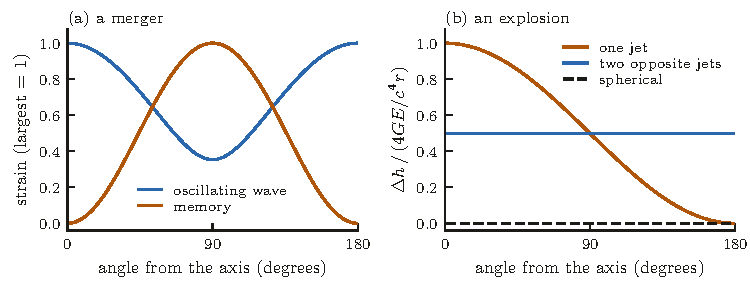
\includegraphics[width=\columnwidth]{figures/memory.pdf}
\caption{The memory, Eq.~\eqref{eq:memory}, against the direction of the
camera. (a) A merger: the oscillating wave is strongest along the orbit's
axis, the memory, Eq.~\eqref{eq:merger-memory}, in its plane. (b) An
explosion whose energy leaves in one jet, in two opposite jets, or evenly in
all directions, in units of $4GE/c^4 r$.}\label{fig:memory}
\end{figure}

\paragraph{The Milky Way.} Tens of millions of close pairs of white dwarfs
radiate at millihertz frequencies; together they make a foreground that will
dominate the sky of the planned space detectors below a few millihertz
\cite{Nelemans2001}. They trace the Galaxy's stars, and averaged over time
and over orientations, which we take to be random, each radiates the same in
every direction; so their brightness on the sky is the column integral of
Eq.~\eqref{eq:column} over a model of the stellar mass, here two exponential discs and a central bulge with masses and
sizes from Bland-Hawthorn and Gerhard \cite{BlandHawthornGerhard2016}. Light
from the same stars passes through a thin disc of dust, which in this model
dims the light of the Galactic centre by about forty magnitudes, comparable
with what is observed. Figure~\ref{fig:milky-way}
shows both on one scale. In light the centre is hardly brighter than the opposite
side of the sky; in gravitational waves it is a hundred times brighter, and
the map is a map of where the Galaxy's stars are. Seeing it this sharply as
a smooth glow would take a camera some $50\,\mathrm{AU}$ across, since at three
millihertz the waves are two-thirds of an astronomical unit long. The pairs are
not a glow, though: after years of observation thousands of the brightest,
above a few millihertz, would each sit alone in its own frequency bin, and a
single pixel could place each of them by Eq.~\eqref{eq:one-wave}, breaking the
smooth map into points.

\begin{figure}
\centering
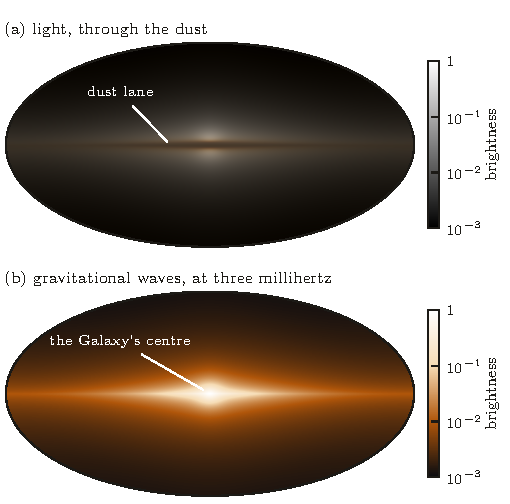
\includegraphics[width=\columnwidth]{figures/milky-way.pdf}
\caption{The Milky Way from the Sun, over the whole sky, centred on the
Galaxy's centre with longitude increasing to the left, both on one logarithmic
scale of brightness. (a) Light from the model's stars, dimmed and reddened by
its dust. (b) Gravitational waves from white-dwarf pairs that trace the same
stars, as an ideal camera about $50\,\mathrm{AU}$ across would see them at
three millihertz. Without its dust, (a) would be identical to (b) in
brightness.}\label{fig:milky-way}
\end{figure}

\paragraph{The first light.} Gravitons stop interacting near the Planck
temperature. If the early universe was ever that hot, they were then in
equilibrium and have kept a black-body spectrum ever since. Every species that
later annihilated heated the photons but not them, so by conservation of
entropy their temperature today is \cite{KolbTurner1990}
\begin{equation}\label{eq:graviton-temperature}
T_g = \left(\frac{3.91}{106.75}\right)^{1/3} T_{\gamma} = 0.905\,\mathrm{K},
\end{equation}
with $T_\gamma = 2.7255\,\mathrm{K}$ \cite{Fixsen2009} and the particles of the
Standard Model; more particles would make it colder. Whether this background
exists is a test of inflation, which would have diluted it away
\cite{VagnozziLoeb2022}. Its energy density counts as $0.05$ of an extra
species of neutrino, within present bounds.

If it exists, it carries more energy than any other background in the
gravitational sky: $7\times10^{-7}$ of the critical density, against about
$10^{-8}$ for the background found by pulsar timing at nanohertz frequencies
\cite{NANOGrav2023}. At high frequencies it outshines everything else in this
paper. A black body of two polarizations sends
$N = 4\zeta(3)(k_BT/h)^3/c^2$ quanta per second per square metre per
steradian: $3.6\times10^{14}$ at $0.905\,\mathrm{K}$, against $6\times10^{-5}$
for the Earth's interior and $4\times10^{5}$ for the Sun's core
(Section~\ref{sec:first-image}). It is also the easiest to image. Its
gravitons are about a centimetre long, so an aperture of a metre resolves a
degree. Four properties follow from what is already known.
\begin{itemize}
\item \emph{It moves with us.} Our motion through it at $370\,\mathrm{km/s}$
\cite{Planck2018I} makes one side of the sky hotter by $v/c = 1.2\times10^{-3}$
of its temperature, exactly as for the microwave background.
\item \emph{On large scales it shares the microwave background's spots.} On scales larger
than the horizon at the time the microwave background was released, the
Boltzmann equation of any massless species reduces to
$\dot\Theta = -\dot\Phi$ ($\Theta$ the fractional change of temperature, $\Phi$ that of the spatial metric), the same for gravitons streaming freely as for
photons held in the plasma. With the same adiabatic start, the two arrive at
that time with the same temperature perturbation, and from then on travel
together through the same potentials. To this approximation the graviton sky
shares the large spots of the microwave sky, from a surface only $2\%$
farther away; how closely, scale by scale, is a question for a
cross-correlation of the two. It differs below a degree or so, where it has no
acoustic peaks, its gravitons never having moved with the plasma, and it is
not smoothed by the diffusion that blurs the microwave sky below a few
arcminutes, since its gravitons never scattered \cite{Bartolo2019}.
\item \emph{Lensing leaves its uniform part unchanged.} Bending conserves
surface brightness, so a uniform background stays uniform however its rays are
bent; only its departures from uniformity, the dipole of our motion and the
spots, are moved about.
\item \emph{Only black holes cast shadows on it.} Nothing else absorbs
appreciably across a broad band (Section~\ref{sec:no-lens}). Seen against this background, the sky is a
uniform glow at $0.905\,\mathrm{K}$, warmer in the direction of our motion,
with a black disc wherever a black hole stands.
\end{itemize}
Figure~\ref{fig:black-hole} computes one such view by exact rays of the
Schwarzschild metric \cite{Darwin1959,Synge1966,Luminet1979}. The camera is at
rest $40\,GM/c^2$ from a black hole that lies just above the Galaxy's centre.
In light, the Milky Way bends around the hole into a ring, with a second image
above it. In primordial gravitons the background is uniform except for the
dipole of our motion, so all that shows is the shadow, of angular radius
$\sin^{-1}[\sqrt{27}\,(GM/c^2 r)\sqrt{1-2GM/c^2 r}] = 7.3^\circ$, and the
dipole folded around it. The whole sky is $2.6\%$ warmer than far from the
hole, $T_g/\sqrt{1-2GM/c^2 r}$, so the camera's thermometer also reads how deep
it sits in the hole's potential.

A black hole is dark against this background only because it is colder. Its
Hawking temperature, $\hbar c^3/8\pi GMk_B$, equals $0.905\,\mathrm{K}$ for a
mass of $1.36\times10^{23}\,\mathrm{kg}$, nearly two masses of the Moon. A
heavier hole casts a shadow; a lighter one glows against the sky; and one of
just this mass, in equilibrium with the background, returns in every mode
exactly what it receives and cannot be seen at all. Spin changes this too. A
spinning hole amplifies the waves that turn with it, by up to $138\%$ for the
most favoured mode of a hole spinning near its limit
\cite{TeukolskyPress1974}, so at wavelengths comparable to its size it would
return more of the background than it receives on that side, and appear
brighter than the sky there rather than dark.

Mode by mode the bookkeeping is exact. A wave of angular degree $l$ and
frequency $\omega$ that reaches the hole is absorbed with probability
$\Gamma_l(\omega)$ and otherwise scattered back, and the hole emits in the
same proportion, so what the camera receives from it in that mode differs
from the sky's occupation $n_{\mathrm{bg}}$ by $\Gamma_l\,(n_H - n_{\mathrm{bg}})$,
with $n_H$ the occupation at the hole's temperature. For a spinning hole
$n_H$ is taken at $\omega - m\Omega_H$, $\Omega_H$ the angular velocity of its
horizon, and in the modes that turn with it faster than it, $\omega <
m\Omega_H$, both factors change sign: whatever the temperatures, those modes
come out brighter than the sky. For a hole that does not spin we have computed
$\Gamma_l$ for every mode from the Regge--Wheeler equation. The shadow is then
less deep than the black disc of the geometric cross-section $27\pi G^2M^2/c^4$
suggests, because the sky's gravitons are not short compared with the hole:
against the $0.905\,\mathrm{K}$ background, a hole ten times the equilibrium
mass is $93\%$ as dark as that disc, three times, $60\%$, and twice, $29\%$;
only above about a hundred times, $10^{25}\,\mathrm{kg}$, is it black. The
reference implementation checks the conservation of flux in every mode,
Page's limit for long waves, $\Gamma_2 \to (256/225)(GM\omega/c^3)^6$
\cite{Page1976}, and the geometric cross-section for short ones.

\begin{figure*}
\centering
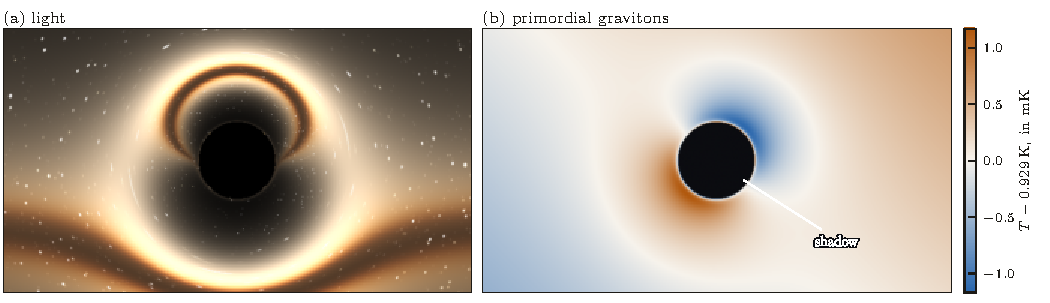
\includegraphics[width=\textwidth]{figures/black-hole.pdf}
\caption{A black hole seen from rest $40\,GM/c^2$ away, through exact
Schwarzschild rays, with the Galaxy's centre $9^\circ$ below the hole. (a) Light:
the model Milky Way of Figure~\ref{fig:milky-way}, with stars added for
orientation, bent into a ring around the shadow and a second image above it.
(b) The primordial graviton background, Eq.~\eqref{eq:graviton-temperature},
warmed to $0.929\,\mathrm{K}$ by the depth of the potential and hotter toward
our direction of motion; the colour shows its departure from the mean, folded
around the shadow by the bending. Nothing else in a gravitational image casts
a shadow.}\label{fig:black-hole}
\end{figure*}

\paragraph{The transparent Sun as a lens.} Gravitational waves pass through
the Sun and, where geometric optics holds, are bent by the mass inside the
cylinder of their impact parameter, $\alpha(b) = 4GM_{\mathrm{cyl}}(b)/c^2 b$.
For Eddington's standard model of the Sun the bending peaks at $4.2''$ for
rays passing $0.28$ of a radius from the centre, more than twice the
$1.75''$ of rays that graze it (Figure~\ref{fig:sun-lens}). Rays through the
centre come to a focus first, $c^2/4\pi G\Sigma(0) = 34\,\mathrm{AU}$ behind
the Sun, where $\Sigma$ is the column density; Patla and Nemiroff found
$23.5\,\mathrm{AU}$ for the denser core of the standard solar model
\cite{PatlaNemiroff2008}. From farther away a compact source directly behind
the Sun appears as a ring inside the solar disc, at the impact parameter
whose focus lies at the camera. A uniform background, such as the primordial
one, is not changed.

Geometric optics needs more than a wavelength shorter than the Sun. A lens of
mass $M$ delays a wave by about $4GM/c^3$, twenty microseconds for the Sun, and
it focuses only if that delay spans a radian or more of the wave's phase, that
is above $c^3/8\pi GM = 8\,\mathrm{kHz}$ for the Sun, whatever its size. Below,
diffraction erases the focus: even a point of the Sun's mass raises the
intensity on its axis only by the factor $\pi w/(1 - e^{-\pi w})$, with $w =
8\pi GMf/c^3$, which is $1.02$ at $100\,\mathrm{Hz}$. The transparent Sun is a
lens for thermal and primordial gravitons, not for the waves of orbiting or
merging bodies.

Wave optics joins the two regimes. For a source directly behind the Sun the
amplitude on the axis, a distance $d$ behind it, is the Fresnel integral over
the plane of the Sun of $e^{ik[b^2/2d - \Phi(b)]}$, where $\Phi' = \alpha$ is
the extra path through its field. Outside the disc $\Phi$ is a point mass's,
and that part of the integral is an incomplete gamma function; inside it is
smooth, and we integrate it numerically. On Earth's orbit the Sun never raises
the intensity by more than the $6\%$ of the central ray's geometric focusing,
$(1 - d/f_0)^{-2}$ with $f_0 = 33.7\,\mathrm{AU}$, which it reaches only above
about $10\,\mathrm{kHz}$. Beyond the central focus a ring of rays from inside
the Sun converges on the axis, and the gain there grows in proportion to the
frequency: at $50\,\mathrm{AU}$ it is $3.4$ at $10\,\mathrm{kHz}$, $44$ at
$100\,\mathrm{kHz}$ and $480$ at $1\,\mathrm{MHz}$, from $1.1$ to $1.25$
times that of a point of the Sun's mass, $\pi w$, and equal to it at
$550\,\mathrm{AU}$, where the converging rays graze the limb. At the
frequencies of thermal gravitons, near $10^{13}\,\mathrm{Hz}$, the same
proportion gives some $5\times10^{9}$. The reference implementation checks the
method against the point mass's closed form, and both limits: long waves,
which see only the Sun's whole mass, and short ones, which follow the rays.

\begin{figure}
\centering
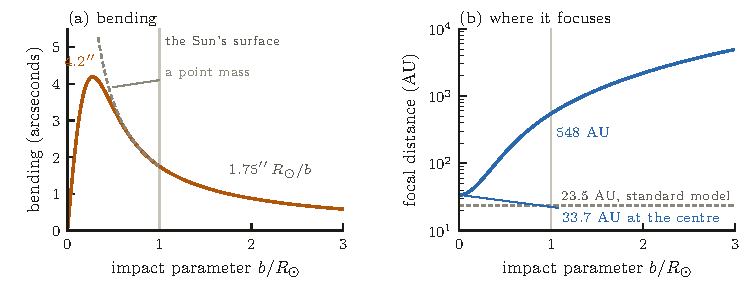
\includegraphics[width=\columnwidth]{figures/sun-lens.pdf}
\caption{The transparent Sun as a lens for gravitational waves, in
Eddington's standard model. (a) Bending against the impact parameter:
inside the Sun it rises to $4.2''$ and falls to zero at the centre; the dashed
curve is what a point mass would give. (b) The distance behind the Sun at
which the rays at each impact parameter cross the axis: $34\,\mathrm{AU}$
through the centre, $548\,\mathrm{AU}$ at the surface. The dashed line marks
the $23.5\,\mathrm{AU}$ found for the standard solar model.}\label{fig:sun-lens}
\end{figure}

\paragraph{Two further consequences.} There is no flash photography. To
light a scene and see what it reflects, matter would have to scatter
gravitational waves, and the cross-section of a body of mass $m$ is of order
$(Gm/c^2)^2$ \cite{Peters1976}, $10^{-50}\,\mathrm{m^2}$ for a person: every
picture in this paper is made by what the scene itself emits or how it pulls.
And an earthquake shows in two parts of the field. Compressional waves change
the density of the rock they cross, and with it $\tE$; that is the prompt
signal already recorded \cite{Vallee2017}. Shear waves in a uniform medium do
not change its density, but they move mass, and so appear in $\tB$, through
Eq.~\eqref{eq:current-column}.
